%% talk1.tex
%% Copyright 2022 Tom M. Ragonneau
%
% This work may be distributed and/or modified under the
% conditions of the LaTeX Project Public License, either version 1.3
% of this license or (at your option) any later version.
% The latest version of this license is in
%   http://www.latex-project.org/lppl.txt
% and version 1.3 or later is part of all distributions of LaTeX
% version 2005/12/01 or later.
%
% This work has the LPPL maintenance status `maintained'.
%
% The Current Maintainer of this work is Tom M. Ragonneau.
\documentclass{polyu-presentation}
\usepackage[final]{microtype}

% List of hyphenation exceptions for US English
% Source: https://ctan.org/tex-archive/info/digests/tugboat/hyphenex
\input{ushyphex}

% Bibliographical resources
\addbibresource{ragonneau-bib/strings.bib}
\addbibresource{ragonneau-bib/optim.bib}

% Dedicated mathematical macros
\newcommand{\con}[1]{c_{#1}}
\newcommand{\ieq}{\mathcal{E}}
\newcommand{\iub}{\mathcal{I}}
\newcommand{\obj}{f}

\title{Model-Based DFO Methods and Software}
\subtitle{Talk no.\ 1 \textemdash\ Overview of DFO}
\author[Tom M. Ragonneau]{Tom M. Ragonneau (\email{tom.ragonneau@polyu.edu.hk})}
\institute[PolyU AMA]{
    Supervised by Dr.\ Zaikun Zhang (\email{zaikun.zhang@polyu.edu.hk})\\
    Co-supervised by Prof.\ Xiaojun Chen (\email{maxjchen@polyu.edu.hk})\and
    Department of Applied Mathematics\\
    The Hong Kong Polytechnic University
}
\date{September 13, 2022}
\titlegraphic{}

\begin{document}

\begin{frame}
	\titlepage
\end{frame}

\begin{frame}
    \frametitle{Table of contents}
	\tableofcontents[hideallsubsections]
\end{frame}

\section{Introduction to DFO}

\begin{frame}
    \frametitle{What is DFO?}

    Derivative-free optimization (DFO) aims at minimizing an objective function~$\obj$ \alert{using function values} but not derivatives.
    The objective function can be a \alert{black box}, resulting from \alert{experiments} or \alert{complex simulations} (PDE, \dots).

    \bigskip

    \begin{center}
        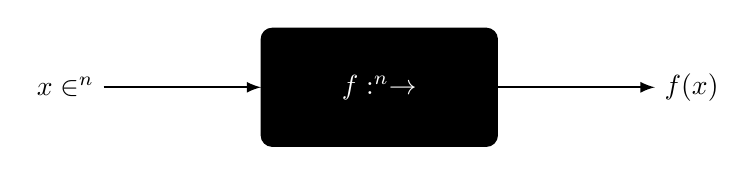
\begin{tikzpicture}
            \draw[thick,-latex] (0,0) -- (2,0);
            \draw[rounded corners,fill=black] (2,-0.75) rectangle (5,0.75);
            \draw[thick,-latex] (5,0) -- (7,0);
            \node[left] at (0,0) {$x \in \R^n$};
            \node at (3.5,0) {\textcolor{white}{$\obj : \R^n \to \R$}};
            \node[right] at (7,0) {$\obj(x)$};
        \end{tikzpicture}
    \end{center}

    \bigskip

    \begin{block}{}
        \begin{enumerate}
            \item The function~$\obj$ may be smooth, but derivatives \alert{cannot be evaluated}.
            \item Each objective function evaluation is \alert{expensive}.
            \item The complexity measure is the \alert{number of function evaluations}.
        \end{enumerate}
    \end{block}
\end{frame}

\begin{frame}
    \frametitle{Fairy tale vs.\ reality}

    \alert<2>{The reality} is often more complex than \alert<1>{the theory}.

    \bigskip
    
    \only<1>{
        \begin{center}
            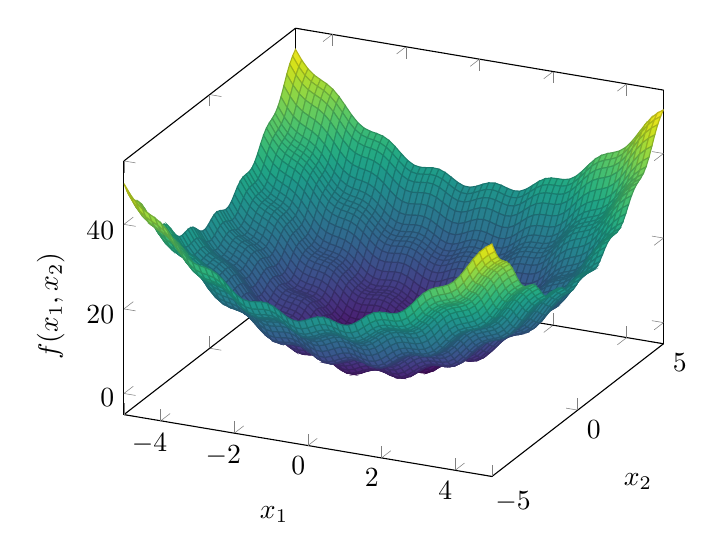
\begin{tikzpicture}
                \begin{axis}[%
                    colormap/viridis,%
                    xmin=-5,%
                    xmax=5,%
                    ymin=-5,%
                    ymax=5,%
                    zmin=-5,%
                    zmax=55,%
                    xlabel={$x_1$},%
                    ylabel={$x_2$},%
                    zlabel={$\obj(x_1, x_2)$},%
                ]
                    \addplot3[%
                        domain=-5:5,%
                        domain y=-5:5,%
                        samples=60,%
                        surf,%
                    ]{x^2+sin(250*x)+y^2+sin(250*y)};
                \end{axis}
            \end{tikzpicture}
        \end{center}
    }
    \only<2>{
        \begin{center}
            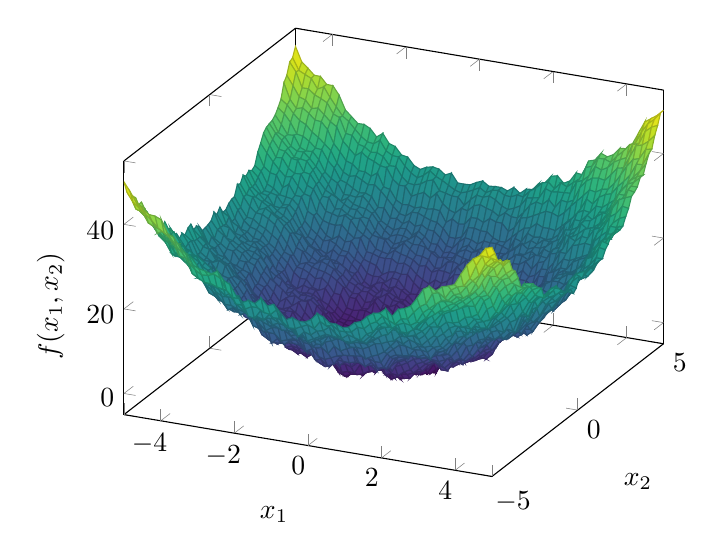
\begin{tikzpicture}
                \begin{axis}[%
                    colormap/viridis,%
                    xmin=-5,%
                    xmax=5,%
                    ymin=-5,%
                    ymax=5,%
                    zmin=-5,%
                    zmax=55,%
                    xlabel={$x_1$},%
                    ylabel={$x_2$},%
                    zlabel={$\obj(x_1, x_2)$},%
                ]
                    \addplot3[%
                        domain=-5:5,%
                        domain y=-5:5,%
                        samples=60,%
                        surf,%
                    ]{x^2+sin(250*x)+y^2+sin(250*y)+rand};
                \end{axis}
            \end{tikzpicture}
        \end{center}
    }
    
\end{frame}

\begin{frame}
    \frametitle{Mathematical formulation}

    The problems we consider are of the form
    \begin{align*}
        \min_{x \in \R^n}   & \quad \obj(x)\\
        \mathrm{s.t.}       & \quad \con{i}(x) \le 0, ~ i \in \iub,\\
                            & \quad \con{i}(x) = 0, ~ i \in \ieq,
    \end{align*}
    where~$\obj : \R^n \to \R$ is the \alert{objective function} and~$\con{i} : \R^n \to \R$ are the \alert{constraint functions} for~$i \in \iub \cup \ieq$, with~$\iub \cap \ieq = \emptyset$.

    \bigskip

    \begin{block}{}
        \begin{enumerate}
            \item The \alert{feasible set} of this problem is
            \begin{equation*}
                \Omega = \set{x \in \R^n : \con{i}(x) \le 0, ~ i \in \iub ~ \mathrm{and} ~ \con{i}(x) = 0, ~ i \in \ieq}
            \end{equation*}
            \item The derivatives of~$\obj$ and~$\con{i}$, with~$i \in \iub \cup \ieq$, are \alert{unknown}.
            \item \alert{No structure} of the problem (e.g., convexity) is assumed.
        \end{enumerate}
    \end{block}
\end{frame}

\section{Examples of applications}

\begin{frame}
    \frametitle{Examples of DFO problems I}

    \begin{block}{Stability of the Gaussian elimination~\parencite{Higham_1993}}
        Given a nonzero matrix~$A \in \R^{n \times n}$, denote by~$a_{i, j}^{(k)}$ the~$(i, j)$th component of the~$k$th matrix of the \alert{Gaussian elimination with partial pivoting}.
        The \alert{stability} of the Gaussian elimination is determined by the \alert{growth factor} of~$A$, given by
        \begin{equation*}
            \rho_n(A) = \frac{\max_{i, j, k} \abs{a_{i, j}^{(k)}}}{\max_{i, j} \abs{a_{i, j}}}.
        \end{equation*}
        By solving
        \begin{equation*}
            \max_{A \in \R^{n \times n}} \rho_n(A),
        \end{equation*}
        we can get insights about the \alert{worst-case scenario} and obtain a starting point for \alert{theoretical analyses}.
    \end{block}

    \bigskip

    What is~\alert{$\nabla \rho_n$}? Does it even exist?
\end{frame}

\begin{frame}
    \frametitle{Examples of DFO problems II}

    To do.
\end{frame}

\section{Optimality conditions for smooth optimization}

\begin{frame}
    \frametitle{Title}
\end{frame}

\section{Methodology of DFO}

\begin{frame}
    \frametitle{Title}
\end{frame}

\section{Benchmarking tools for DFO methods}

\begin{frame}
    \frametitle{Title}

    \parencite{Dolan_More_2002,More_Wild_2009,Gould_Scott_2016}
\end{frame}

\appendix

\begin{frame}[t,allowframebreaks]
    \frametitle{References}

	\printbibliography
\end{frame}

\end{document}